%\title{beavtex}
\documentclass[double,12pt]{beavtex}
\usepackage{graphicx}
\usepackage{rotating} %Package added to allow the rotation of figures and chart on a page, {sidewaysfigure} command
\usepackage{tablefootnote} %Packaged added to allow footnotes in the tabular environment, use \tablefootnote command
\usepackage[round]{natbib}
\usepackage{booktabs}
\bibliographystyle{plainnat}
\title{An Analysis of Something}
\author{Joseph A. Student}
\degree{Master of Science}
\doctype{Thesis}
\department{Nuclear Engineering and Radiation Health Physics}
\depttype{School}
\depthead{Director}
\major{Radiation Health Physics}
\advisor{Jane R. Professor}
\advisor{Jane D. Professor}
\submitdate{January 1, 2013}
\commencementyear{2013}


\abstract{This is the place for the abstract text.}


\acknowledgements{I would like to acknowledge...Lorem ipsum dolor sit amet, consectetur adipiscing elit. Maecenas vel eros sed mauris porttitor semper nec a orci. Nullam vestibulum mi nec condimentum posuere. Pellentesque eget diam id sapien aliquet ullamcorper. Pellentesque blandit nec lectus ut mollis. Praesent in facilisis justo. Vestibulum ante ipsum primis in faucibus orci luctus et ultrices posuere cubilia Curae; Sed eget congue leo, sed consequat libero. In rutrum malesuada nisi. Vestibulum ante ipsum primis in faucibus orci luctus et ultrices posuere cubilia Curae; Morbi sollicitudin tortor ut sem facilisis mollis.}


\begin{document}
\maketitle
\mainmatter

%-------------------------INTRODUCTION-----------------------------

\chapter{Introduction}

\section{Objective}


The Douglas-fir forests of the coastal Pacific Northwest are among the most productive globally ~\citep{mcardleYieldDouglasFir1930,waringEvergreenConiferousForests1979,HermanLavender1999}. Maintaining forest productivity of this region is important for the continued viability of the Pacific Northwest timber industry, as well as for its potential to regulate atmospheric carbon in the ongoing climate crisis. This productivity is due to a combination of high soil nitrogen (N) and climate that is favorable to tree growth. Whereas the majority of forests worldwide are N limited due to low N availability, the coastal Douglas-fir forests  have undergone centuries of N saturation due to historic presence of the symbiotic N-fixing red alder (*Alnus rubra*) in the region ~\citep{binkley1983}. When soil N availability comes to exceed tree requirements, tree growth commonly becomes limited by other nutrients required in high quantities to sustain growth, such as P, Ca, K, and S ~\citep{mainwaringThreeyearGrowthResponse2014, perakisForestCalciumDepletion2013, turnerUseFoliageSulphate1977, radwanNutritionDouglasfir}. 

When soil N supply exceeds ecosystem N demand, N saturation is known to occur ~\citep{agrenNitrogenSaturationTerrestrial1988}. Highly N saturated soils undergo enhanced soil nitrification and subsequent coupled nitrate-base cation leaching ~\citep{perakisCoupledNitrogenCalcium2006}. Nitrification particularly accelerates calcium (Ca) and magnesium (Mg) losses from soils ~\citep{homann1994}. As Ca is required in higher quantities by trees than Mg, and is known to be distinctly limiting in forests predisposed to highly acidic and weathered soil conditions ~\citep{likensHB1998, federerLongtermDepletionCalcium1989, bigelowNutrientLimitationJuvenile2007}, it is more likely that Ca deficiency is to develop in the higher N soils of the Oregon Coast Range (OCR) rather than other base cations. In contrast to accelerated leaching losses, chronic N saturation and nitrification can stimulate accelerated mineral weathering ~\citep{berthelinMajorRoleNitrification1985, PerakisPettRidge2019}. However, over millennia, the  source of ecosystem Ca supply in the OCR has shifted from mineral to atmospheric in soils with either sedimentary or basaltic soil minerals. This implies either a depletion or an inaccessibility of the weatherable pool of nutrient cations at N saturated sites ~\citep{hynicka2016, leysNaturalAnthropogenicDrivers2016a}. Despite a large disparity between potential base cation supply between soil minerals in OCR soils, chronic N saturation may nevertheless lead to base cation limitations all forests. 

Although ecosystem nutrient cycling processes are sufficient in supplying Ca in many unaltered forests ~\citep{vitousekLitterfallNutrientCycling1984, hiltonNutrientCyclingTropical1987}, a large portion of Douglas-fir in the OCR is specifically grown for the harvest of timber. Removals of tree nutrients through harvest is a primary cause of ecosystem nutrient losses in managed forests ~\citep{johnsonSymposiumForestSite1986}, and may quickly lead to soil Ca depletion and subsequent forest productivity losses in Ca deficient forests ~\citep{federerLongtermDepletionCalcium1989, nykvistTropicalForestsCan2000}. Intensive forest-harvest practices, such as whole-tree-harvest (WTH), are known to be the major cause of nutrient losses in a range of forest plantations in comparison to moderate practices, such as bole-only (BOH) harvest  ~\citep{achatQuantifyingConsequencesRemoving2015}. Recent intensification of forest management to improve economic returns has led to shorter rotation schedules of 40 years and lower ~\citep{diazTradeoffsTimberCarbon2018}, with potential to accelerate nutrient removals substantially. It is estimated that high N Douglas-fir forests under WTH will reach soil Ca depletion within ~50 years of continued harvest, whereas the application of BOH can extend this to ~400 years ~\citep{perakisCoupledNitrogenCalcium2006}. However, it remains unknown how many short-rotation harvests must occur to cause nutrient depletion under a variety of soil nutrient conditions.  In Coastal Douglas-fir forests, it is likely to depend on the interaction of harvest intensity and how forest N saturation influences Ca supply from mineral weathering and exchangeable nutrient supply. 

As an analysis of nutrient depletion in the OCR requires the observation of soil nutrient conditions from 40 to 500 years in the future ~\citep{perakisCoupledNitrogenCalcium2006}, a dynamic modelling approach is used to  observe the potential for soil N saturation and harvest to drive nutrient depletion in soils. Relatively few dynamic models of forest nutrient cycling contain sufficient chemical detail to evaluate interactions between nitrogen cycling and calcium supply from mineral weathering. One such model is called “Nutrient Cycling in Forest Ecosystems”, or NutsFor. NutsFor is one of several dynamic process-oriented models that was developed to simulate forest-soil chemical responses to harvest and acidic deposition (van der Heijden et al., 2017). It is a hybrid of the Nutrient Cycling Model (NuCM), the ForSAFE model, and the PROFILE model, which have been used to study base cation nutrient depletion due to acidic deposition and harvest intensity (Verburg et al., 2001; van der Heijden et al., 2011; Liu et al., 1991). NutsFor has adopted NuCM’s exchange site simulations and N-transformation processes, while adding the PROFILE soil mineral weathering model (van der Heijden et al. 2017). NutsFor’s ability to link soil N transformations to soil acidification, mineral weathering, forest management, and exchange site depletion of base cations makes NutsFor well suited to the study of nutrient cycling and depletion in the biogeochemically diverse, intensively managed coastal forests of the PNW. 

In this study, we report how extreme soil N enrichment affects long-term nutrient retention in OCR forests under repeated harvest. We further describe how bedrock type interacts with soil N to supply base cation nutrients to forests. We studied the effects that soil N extremes (low to high) have on nutrient limitation on forests sites overlying either sedimentary or basaltic minerals, over a range of harvest intensities to answer the following questions: Q1: How does soil N saturation affect nutrient losses (especially Ca) in coastal Douglas-fir stands? Q2: How do different stand rotation lengths and harvest types change the rate at which nutrient depletion occurs? Q3: How do different kinds of bedrock (basaltic versus sedimentary) and associated soil minerals influence the rate of nutrient depletion? Q5: When (after how many harvests) do nutrient losses cause biomass accrual rates to slow?



\section{Background}

Lorem ipsum dolor sit amet, consectetur adipiscing elit. Sed venenatis nunc sapien. Praesent imperdiet nulla eu rutrum venenatis. Fusce rhoncus urna a nunc semper, non venenatis lorem tempor. Cras sollicitudin eget velit eu venenatis. Mauris imperdiet pretium massa sed dapibus. Nunc ipsum ipsum, porttitor ut urna ut, pretium feugiat leo. Nunc magna enim, facilisis a porttitor eget, elementum ac turpis. Quisque et gravida justo. Etiam vulputate quam at commodo suscipit. Vivamus ut adipiscing tortor. Phasellus quis dolor et mi hendrerit sollicitudin. 

Cras dapibus congue mauris, et imperdiet magna pellentesque non. Sed venenatis adipiscing quam ut placerat. Praesent imperdiet dignissim cursus. Phasellus mattis nibh vitae semper pellentesque. Lorem ipsum dolor sit amet, consectetur adipiscing elit. Sed dignissim tellus id adipiscing tempus. Aenean posuere malesuada rhoncus. Ut quis elit eros.



%------------------------LIT REVIEW--------------------------------

\chapter{Literature Review}

\section{First Section of Lit Review}

Frogs are weird...

\begin{figure}[ht!]
\begin{center}
	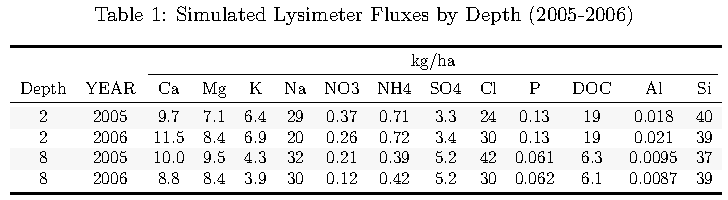
\includegraphics[width=20cm]{Images/LN_SED/Base/test.pdf}
	\caption{Frog pic...}
	\label{fig:frog}
	\end{center}
\end{figure}


Here is a reference to the from pic: Figure~\ref{fig:frog}.

\section{Just another section of this chapter.}

Lorem ipsum dolor sit amet, consectetur adipiscing elit. Sed venenatis nunc sapien. Praesent imperdiet nulla eu rutrum venenatis. Fusce rhoncus urna a nunc semper, non venenatis lorem tempor. Cras sollicitudin eget velit eu venenatis. Mauris imperdiet pretium massa sed dapibus. Nunc ipsum ipsum, porttitor ut urna ut, pretium feugiat leo. Nunc magna enim, facilisis a porttitor eget, elementum ac turpis. Quisque et gravida justo. Etiam vulputate quam at commodo suscipit. Vivamus ut adipiscing tortor. Phasellus quis dolor et mi hendrerit sollicitudin. 

Cras dapibus congue mauris, et imperdiet magna pellentesque non. Sed venenatis adipiscing quam ut placerat. Praesent imperdiet dignissim cursus. Phasellus mattis nibh vitae semper pellentesque. Lorem ipsum dolor sit amet, consectetur adipiscing elit. Sed dignissim tellus id adipiscing tempus. Aenean posuere malesuada rhoncus. Ut quis elit eros.



%-------------------MATERIALS & METHODS--------------------------

\chapter{Materials and Methods}

\section{Primary Methods}

Lorem ipsum dolor sit amet, consectetur adipiscing elit. Sed venenatis nunc sapien. Praesent imperdiet nulla eu rutrum venenatis. Fusce rhoncus urna a nunc semper, non venenatis lorem tempor. Cras sollicitudin eget velit eu venenatis. Mauris imperdiet pretium massa sed dapibus. Nunc ipsum ipsum, porttitor ut urna ut, pretium feugiat leo. Nunc magna enim, facilisis a porttitor eget, elementum ac turpis. Quisque et gravida justo. Etiam vulputate quam at commodo suscipit. Vivamus ut adipiscing tortor. Phasellus quis dolor et mi hendrerit sollicitudin. 

Cras dapibus congue mauris, et imperdiet magna pellentesque non. Sed venenatis adipiscing quam ut placerat. Praesent imperdiet dignissim cursus. Phasellus mattis nibh vitae semper pellentesque. Lorem ipsum dolor sit amet, consectetur adipiscing elit. Sed dignissim tellus id adipiscing tempus. Aenean posuere malesuada rhoncus. Ut quis elit eros.


\begin{table}[ht]
\caption{Types of stuff you put in a table} % title of Table
\centering  % used for centering table
\begin{tabular}{c c} % centered columns (2 columns)
\hline\hline                        %inserts double horizontal lines
Header 1 & Header 2 \\ [0.5ex] % inserts table heading
\hline                  % inserts single horizontal line
Item 1 & something  \\ % inserting body of the table
Item 2 & something else  \\
Item 3 & more things  \\
Item 4 & and more \\
Item 5 & last thing \\ [1ex]      % [1ex] adds vertical space
\hline %inserts single line
\end{tabular}
\label{table:misc} % is used to refer this table in the text
\end{table}


\begin{table}[ht]
\centering
\caption{Thicker horizontal lines above and below the table.}
\begin{tabular}[t]{lcc}
\toprule
&Treatment A&Treatment B\\
\midrule
John Smith&1&2\\
Jane Doe&--&3\\
Mary Johnson&4&5\\
\bottomrule
\end{tabular}
\end{table}%


\section{More Methods}

Lorem ipsum dolor sit amet, consectetur adipiscing elit. Sed venenatis nunc sapien. Praesent imperdiet nulla eu rutrum venenatis. Fusce rhoncus urna a nunc semper, non venenatis lorem tempor. Cras sollicitudin eget velit eu venenatis. Mauris imperdiet pretium massa sed dapibus. Nunc ipsum ipsum, porttitor ut urna ut, pretium feugiat leo. Nunc magna enim, facilisis a porttitor eget, elementum ac turpis. Quisque et gravida justo. Etiam vulputate quam at commodo suscipit. Vivamus ut adipiscing tortor. Phasellus quis dolor et mi hendrerit sollicitudin. 

Cras dapibus congue mauris, et imperdiet magna pellentesque non. Sed venenatis adipiscing quam ut placerat. Praesent imperdiet dignissim cursus. Phasellus mattis nibh vitae semper pellentesque. Lorem ipsum dolor sit amet, consectetur adipiscing elit. Sed dignissim tellus id adipiscing tempus. Aenean posuere malesuada rhoncus. Ut quis elit eros.


%------------------------RESULTS--------------------------------

\chapter{Results}

Lorem ipsum dolor sit amet, consectetur adipiscing elit. Fusce posuere sed magna sit amet hendrerit. Integer gravida mattis posuere. Pellentesque at libero consectetur, pulvinar augue ac, pharetra augue. Cras fermentum augue id odio rutrum, eget eleifend lectus adipiscing. Duis libero massa, rutrum eget purus eu, tempus dapibus dolor. Class aptent taciti sociosqu ad litora torquent per conubia nostra, per inceptos himenaeos. Sed aliquet fringilla odio at euismod. Etiam viverra convallis tortor, hendrerit varius nulla pharetra ac. 

Donec vitae mollis sem, non viverra arcu. Integer vel risus justo. Proin consectetur justo nisl, ut auctor mauris rhoncus id. Vestibulum eget egestas risus. Nullam eget nunc non tortor pretium rhoncus dapibus eu orci. In hendrerit velit vel turpis vulputate porttitor. Praesent commodo, neque at porta posuere, ligula ipsum euismod dolor, ac pharetra erat purus non nunc. Praesent placerat placerat fermentum. Class aptent taciti sociosqu ad litora torquent per conubia nostra, per inceptos himenaeos. Praesent volutpat, purus id molestie egestas, mauris neque accumsan tellus, vitae fermentum lorem neque a lectus. Morbi tincidunt metus dui, vitae adipiscing mauris porttitor vitae. Donec a dolor convallis, tincidunt sapien vel, malesuada lorem. Fusce a magna sit amet leo accumsan dapibus at nec tellus. Nam id erat at ligula adipiscing porttitor in semper augue. Etiam imperdiet lobortis dui, a ornare lorem vulputate vitae. 

Etiam non libero in leo egestas porta et eu nunc. Duis molestie suscipit semper. Vestibulum nec sodales odio, vestibulum sagittis lacus. Phasellus volutpat, velit in pretium malesuada, nibh magna consequat neque, in interdum magna mi at erat. In hac habitasse platea dictumst. Praesent consectetur ut lorem sagittis tempus. Ut venenatis eu mi eget sollicitudin. Praesent posuere non lorem nec lacinia. Nunc at vulputate dolor. Aliquam et dolor sit amet quam viverra condimentum vitae eu dui. Quisque pellentesque purus in tortor vehicula sollicitudin. Curabitur sit amet vehicula diam. Vivamus mauris nulla, dictum ac ipsum eget, molestie scelerisque diam. Curabitur sit amet dolor nibh. Cum sociis natoque penatibus et magnis dis parturient montes, nascetur ridiculus mus. Sed semper sed diam quis feugiat. 


\begin{equation}
MDC=\frac{3.29*\sqrt{(Bkgcpm*C_{t}*(1+\frac{C_{t}}{BkgC_{t}}))}+3.0}{2.22*E*C_{t}*V*decay*A*R*DF*I}
\label{eq:mdc}
\end{equation}
Where:

\begin{itemize}
\item $C_{t} =$ Sample count time
\item $BkgC_{t} =$ Background count time
\item $Bkgcpm =$ Background counts per minute (cpm)
\item $E =$ Counting efficiency
\item $V =$ Sample volume or weight
\item $decay =$ isotopic decay (if applicable)
\item $A =$ Isotopic abundance (if applicable)
\item $R =$ Recovery (if applicable)
\item $DF =$ Dilution factor for liquid scintillation (if applicable)
\item $I =$ Additional decay or ingrowth factors (if applicable)
\end{itemize}

Lorem ipsum dolor sit amet, consectetur adipiscing elit. Sed venenatis nunc sapien. Praesent imperdiet nulla eu rutrum venenatis. Fusce rhoncus urna a nunc semper, non venenatis lorem tempor. Cras sollicitudin eget velit eu venenatis. Mauris imperdiet pretium massa sed dapibus. Nunc ipsum ipsum, porttitor ut urna ut, pretium feugiat leo. Nunc magna enim, facilisis a porttitor eget, elementum ac turpis. Quisque et gravida justo. Etiam vulputate quam at commodo suscipit. Vivamus ut adipiscing tortor. Phasellus quis dolor et mi hendrerit sollicitudin. 

Cras dapibus congue mauris, et imperdiet magna pellentesque non. Sed venenatis adipiscing quam ut placerat. Praesent imperdiet dignissim cursus. Phasellus mattis nibh vitae semper pellentesque. Lorem ipsum dolor sit amet, consectetur adipiscing elit. Sed dignissim tellus id adipiscing tempus. Aenean posuere malesuada rhoncus. Ut quis elit eros.


\pagebreak[4]

\begin{figure}
\begin{center}
	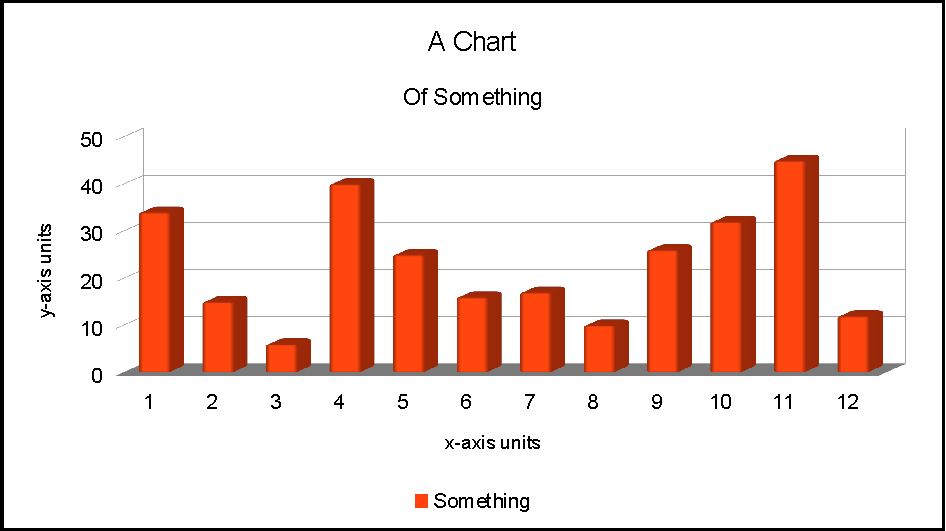
\includegraphics[width=14cm]{chart.pdf}
	\caption{A Chart.}
	\label{fig:chart}
	\end{center}
\end{figure}

\pagebreak[4]

\begin{sidewaysfigure}[htbp]
\begin{center}
	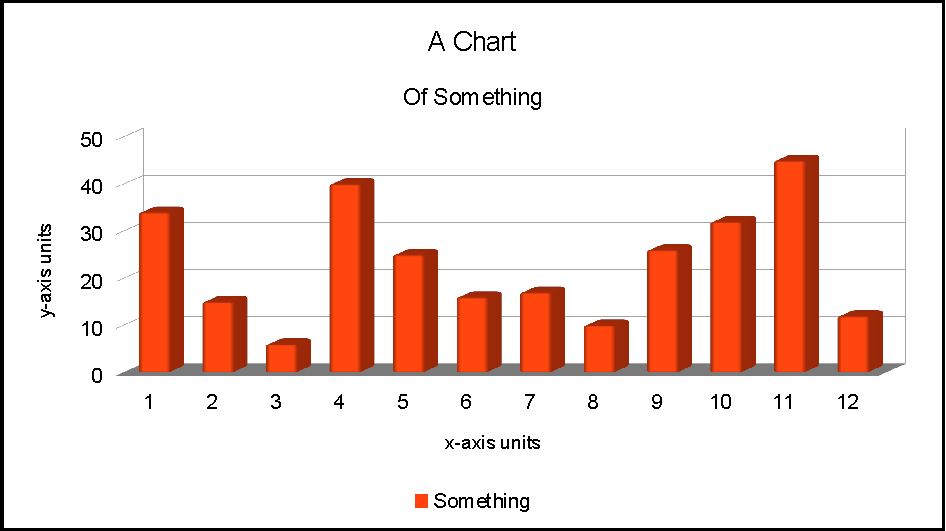
\includegraphics[width=18cm]{chart.pdf}
	\caption{Same chart, but using sidewaysfigure.}
	\label{fig:rain}
	\end{center}
\end{sidewaysfigure}


%-----------------------DISCUSSION--------------------------------

\chapter{Discussion}

\section{First Subsection}

Lorem ipsum dolor sit amet, consectetur adipiscing elit. Fusce posuere sed magna sit amet hendrerit. Integer gravida mattis posuere. Pellentesque at libero consectetur, pulvinar augue ac, pharetra augue. Cras fermentum augue id odio rutrum, eget eleifend lectus adipiscing. Duis libero massa, rutrum eget purus eu, tempus dapibus dolor. Class aptent taciti sociosqu ad litora torquent per conubia nostra, per inceptos himenaeos. Sed aliquet fringilla odio at euismod. Etiam viverra convallis tortor, hendrerit varius nulla pharetra ac. 

Donec vitae mollis sem, non viverra arcu. Integer vel risus justo. Proin consectetur justo nisl, ut auctor mauris rhoncus id. Vestibulum eget egestas risus. Nullam eget nunc non tortor pretium rhoncus dapibus eu orci. In hendrerit velit vel turpis vulputate porttitor. Praesent commodo, neque at porta posuere, ligula ipsum euismod dolor, ac pharetra erat purus non nunc. Praesent placerat placerat fermentum. Class aptent taciti sociosqu ad litora torquent per conubia nostra, per inceptos himenaeos. Praesent volutpat, purus id molestie egestas, mauris neque accumsan tellus, vitae fermentum lorem neque a lectus. Morbi tincidunt metus dui, vitae adipiscing mauris porttitor vitae. Donec a dolor convallis, tincidunt sapien vel, malesuada lorem. Fusce a magna sit amet leo accumsan dapibus at nec tellus. Nam id erat at ligula adipiscing porttitor in semper augue. Etiam imperdiet lobortis dui, a ornare lorem vulputate vitae. 

Etiam non libero in leo egestas porta et eu nunc. Duis molestie suscipit semper. Vestibulum nec sodales odio, vestibulum sagittis lacus. Phasellus volutpat, velit in pretium malesuada, nibh magna consequat neque, in interdum magna mi at erat. In hac habitasse platea dictumst. Praesent consectetur ut lorem sagittis tempus. Ut venenatis eu mi eget sollicitudin. Praesent posuere non lorem nec lacinia. Nunc at vulputate dolor. Aliquam et dolor sit amet quam viverra condimentum vitae eu dui. Quisque pellentesque purus in tortor vehicula sollicitudin. Curabitur sit amet vehicula diam. Vivamus mauris nulla, dictum ac ipsum eget, molestie scelerisque diam. Curabitur sit amet dolor nibh. Cum sociis natoque penatibus et magnis dis parturient montes, nascetur ridiculus mus. Sed semper sed diam quis feugiat. 

\begin{equation}
A(t)=A_{o}e^{(-\lambda t)}
\label{eq:initialeq}
\end{equation}

Then Equation~\ref{eq:initialeq} is integrated to become:

\begin{equation}
\tilde{C}=\int_0^{t}A(t)dt = \frac{A_{o}}{\lambda} (1-e^{(-\lambda t)})
\label{eq:finaleq}
\end{equation}

Where:

\begin{itemize}
\item $A(t) =$ original exponential function
\item $A_{o} =$ the peak activity at day 0 (Bq per mass or volume)
\item $\tilde{C} =$ Integrated Activity Concentration (Bq-days per mass or volume)
\item $t =$ 28 days
\item $\lambda =$ removal constant (day$^{-1}$)
\end{itemize}



\section{Another Subsection}

Lorem ipsum dolor sit amet, consectetur adipiscing elit. Fusce posuere sed magna sit amet hendrerit. Integer gravida mattis posuere. Pellentesque at libero consectetur, pulvinar augue ac, pharetra augue. Cras fermentum augue id odio rutrum, eget eleifend lectus adipiscing. Duis libero massa, rutrum eget purus eu, tempus dapibus dolor. Class aptent taciti sociosqu ad litora torquent per conubia nostra, per inceptos himenaeos. Sed aliquet fringilla odio at euismod. Etiam viverra convallis tortor, hendrerit varius nulla pharetra ac. 

Donec vitae mollis sem, non viverra arcu. Integer vel risus justo. Proin consectetur justo nisl, ut auctor mauris rhoncus id. Vestibulum eget egestas risus. Nullam eget nunc non tortor pretium rhoncus dapibus eu orci. In hendrerit velit vel turpis vulputate porttitor. Praesent commodo, neque at porta posuere, ligula ipsum euismod dolor, ac pharetra erat purus non nunc. Praesent placerat placerat fermentum. Class aptent taciti sociosqu ad litora torquent per conubia nostra, per inceptos himenaeos. Praesent volutpat, purus id molestie egestas, mauris neque accumsan tellus, vitae fermentum lorem neque a lectus. Morbi tincidunt metus dui, vitae adipiscing mauris porttitor vitae. Donec a dolor convallis, tincidunt sapien vel, malesuada lorem. Fusce a magna sit amet leo accumsan dapibus at nec tellus. Nam id erat at ligula adipiscing porttitor in semper augue. Etiam imperdiet lobortis dui, a ornare lorem vulputate vitae. 

Finally, a table with a footnote...

\begin{table}[htbp!]
\caption{Some table values}
\centering
\begin{tabular}{cccccc}
\hline\hline
 & & & & & Total \\
Sample & $A_{o}$\tablefootnote{some kind of footnote from a table, which doesn't work without the tablefootnote package} & $\lambda$ & $\tilde{C}$ & Something & (units) \\
\hline   \\
Item 1 & 1 & .55 & 3 & 125 & 70  \\
Item 2 & 1 & .55 & 3 & 125 & 70  \\
Item 3 & 1 & .55 & 3 & 125 & 70  \\
Item 4 & 1 & .55 & 3 & 125 & 70  \\ [1ex]
\hline
\textbf{Total} &  &  &  &  & \textbf{280} \\ [1ex]
\hline
\end{tabular}
\label{table:intake2}
\end{table}


Etiam non libero in leo egestas porta et eu nunc. Duis molestie suscipit semper. Vestibulum nec sodales odio, vestibulum sagittis lacus. Phasellus volutpat, velit in pretium malesuada, nibh magna consequat neque, in interdum magna mi at erat. In hac habitasse platea dictumst. Praesent consectetur ut lorem sagittis tempus. Ut venenatis eu mi eget sollicitudin. Praesent posuere non lorem nec lacinia. Nunc at vulputate dolor. Aliquam et dolor sit amet quam viverra condimentum vitae eu dui. Quisque pellentesque purus in tortor vehicula sollicitudin. Curabitur sit amet vehicula diam. Vivamus mauris nulla, dictum ac ipsum eget, molestie scelerisque diam. Curabitur sit amet dolor nibh. Cum sociis natoque penatibus et magnis dis parturient montes, nascetur ridiculus mus. Sed semper sed diam quis feugiat.




\chapter{Conclusion}

Lorem ipsum dolor sit amet, consectetur adipiscing elit. Fusce posuere sed magna sit amet hendrerit. Integer gravida mattis posuere. Pellentesque at libero consectetur, pulvinar augue ac, pharetra augue. Cras fermentum augue id odio rutrum, eget eleifend lectus adipiscing. Duis libero massa, rutrum eget purus eu, tempus dapibus dolor. Class aptent taciti sociosqu ad litora torquent per conubia nostra, per inceptos himenaeos. Sed aliquet fringilla odio at euismod. Etiam viverra convallis tortor, hendrerit varius nulla pharetra ac. 

Donec vitae mollis sem, non viverra arcu. Integer vel risus justo. Proin consectetur justo nisl, ut auctor mauris rhoncus id. Vestibulum eget egestas risus. Nullam eget nunc non tortor pretium rhoncus dapibus eu orci. In hendrerit velit vel turpis vulputate porttitor. Praesent commodo, neque at porta posuere, ligula ipsum euismod dolor, ac pharetra erat purus non nunc. Praesent placerat placerat fermentum. Class aptent taciti sociosqu ad litora torquent per conubia nostra, per inceptos himenaeos. Praesent volutpat, purus id molestie egestas, mauris neque accumsan tellus, vitae fermentum lorem neque a lectus. Morbi tincidunt metus dui, vitae adipiscing mauris porttitor vitae. Donec a dolor convallis, tincidunt sapien vel, malesuada lorem. Fusce a magna sit amet leo accumsan dapibus at nec tellus. Nam id erat at ligula adipiscing porttitor in semper augue. Etiam imperdiet lobortis dui, a ornare lorem vulputate vitae. 

Etiam non libero in leo egestas porta et eu nunc. Duis molestie suscipit semper. Vestibulum nec sodales odio, vestibulum sagittis lacus. Phasellus volutpat, velit in pretium malesuada, nibh magna consequat neque, in interdum magna mi at erat. In hac habitasse platea dictumst. Praesent consectetur ut lorem sagittis tempus. Ut venenatis eu mi eget sollicitudin. Praesent posuere non lorem nec lacinia. Nunc at vulputate dolor. Aliquam et dolor sit amet quam viverra condimentum vitae eu dui. Quisque pellentesque purus in tortor vehicula sollicitudin. Curabitur sit amet vehicula diam. Vivamus mauris nulla, dictum ac ipsum eget, molestie scelerisque diam. Curabitur sit amet dolor nibh. Cum sociis natoque penatibus et magnis dis parturient montes, nascetur ridiculus mus. Sed semper sed diam quis feugiat. 

\pagebreak

\bibliography{thesis}

\pagebreak

\appendix

\begin{table}[ht]
\centering
\caption{Sources of Parameterization}
\begin{tabular}[t]{cc}
\toprule
Parameter&Source\\
\midrule
Example Parameter& \cite{bockheimNutrientDynamicsDecomposing2011}\\
Example 2&3\\
4&5\\
\bottomrule
\end{tabular}
\end{table}%

\chapter{Things}





\chapter{More Things}





\end{document}